% From mitthesis package
% Version: 1.10, 2025/04/27
% Documentation: https://ctan.org/pkg/mitthesis


\chapter{Introduction}

% terms:
% - workload = the bundle of endpoints/functions that are running in the same container/isolation entity
% - process = a literal linus process
% - entity = linux term: a runnable thing, either process or a cgroup that contains processes


The benefits of best effort (BE) workloads are clear: in an ideal world, BE has
no latency impact when latency critical workloads have load, but can run
opportunistically and therbey maintain high utilization when there is nothing
else to run. 

In order to reap these benefits, the underlying scheduler needs to be able to
support dynamic reallocation of CPUs. Most workloads on modern servers run in
some sort of isolation context, usually either in VMs or containers, that is
used to isolate access to CPU as well as other resources. Both containers and
VMs rely on the underlying OS to mechanistically enforce the CPU allocation.
Linux is by far the most commmon operating system for servers, and uses
\cgroups{} as the interface to specify resource requirements.
% https://en.wikipedia.org/wiki/Usage_share_of_operating_systems
\hmng{awk, but I think saying the things that need to be said. Flow needs to be
cleaner}

\section{The \cgroups{} interface}

\cgroups{} are a Linux construct that group processes. This allows resource
restrictions apply to the group rather than individual processes. When processes
spawn threads/new processes, those are by default in the same group.

Users specify the resources that each group should get via interface files that
Linux exposes in a pseudo-filesystem (at \texttt{/sys/fs/cgroup}). There are
many different resource constraints that can be placed on a group, for many
different resources (\eg{} cpu, memory, i/o). For specifying cpu resources,
there are three main interface files that control the cpu allocation in
different ways:
\begin{enumerate}
    \item \texttt{cpu.max}: specified using two numbers: \textit{max} and \textit{period}. Linux
    enforces that the group is only allowed to use \textit{max} runtime in \textit{period} time.
    \item \texttt{cpu.weight}: a single number, in the range [1, 10000]. This
    sets the relative weight of the group.
    \item \texttt{cpu.idle}: 0 or 1, this sets the \textit{scheduling policy} of
    the group to be \schedidle{}.
\end{enumerate}

We discuss what exactly scheduling policies are and how they affect the
scheduler in chapter \ref{chp:sched_idle}; since the cpu.idle \cgroups{}
interface file is relatively new (added in 2021), the software discussed below
does not yet support setting this. Thus the main interface files that are used
by existing software isolation systems are \texttt{cpu.max} and
\texttt{cpu.weight}.

\section{How containers use \cgroups{} to dyanimically isolate BE workloads}

Containerization systems consist of two pieces: a low-level runtime, which is in
charge of actually creating and starting the containers, and a high-level
engine, which manages the containers and other metadata. Examples of low-level
runtimes include runc and crun; popular high-level engines include Docker,
Podman, containerd, and CRI-O. The low-level runtime and high-level engine
communicate via a well-defined and standardized interface, specified in the Open
Container Initiative (OCI). The standardized interface allows different engines
to support out different low-level runtimes without needing specialized code for
each.

The OCI has different interfaces for different operating systems, but for Linux
specifies that \cgroups{} is used to `restrict resource usage for a container'.
Each container gets its own group, and resource restrictions/requirements are
enforced by writing the desired values to the relevant \cgroups{} interface
files. Any process or thread that is then started in the container (\ie{} group)
stays within the same group and is subject to the same restrictions.

We look at Kubernetes as a representative example, to understand how resource
requirements specified by the developers are translated into the \cgroups{}
interface.

% OCI interface
% - https://github.com/opencontainers/runtime-spec/blob/main/config-linux.md
% - https://github.com/opencontainers/runtime-spec/blob/main/spec.md

% runc
% - https://github.com/canonical/runc-app/blob/master/docs/systemd.md
% - https://github.com/opencontainers/runc/blob/main/docs/cgroup-v2.md

% crun
% - https://www.redhat.com/en/blog/introduction-crun

% containerd: 
% - https://github.com/containerd/containerd/blob/main/docs/getting-started.md 

% docker: 
% - https://dev.to/mochafreddo/understanding-docker-containers-leveraging-linux-kernels-namespaces-and-cgroups-4fkk
% - https://docs.docker.com/engine/daemon/alternative-runtimes/
% - https://docs.docker.com/engine/containers/resource_constraints/

% podman
% - https://docs.podman.io/en/latest/

% general overviews:
% - https://www.aquasec.com/blog/container-isolation-techniques/
% - https://www.aquasec.com/cloud-native-academy/container-security/container-runtime/
% - https://www.cloudraft.io/blog/container-runtimes
% - https://www.wiz.io/academy/container-runtimes


\subsection{how \cgroups{} are used in Kubernetes}

Kubernetes\cite{kubernetes} allows users to specify cpu resource
requirements in two ways: requests and limits. Limits are directly passed on to
the \cgroups{} cpu.limit interface. Linux implements cpu limits using accounting to
ensure that the processes in the cgroup get no more cpu time than
allowed.

For Kubernetes' resource requests interface, it is desirable that containers be
allowed to burst when possible. For example, a service $s_1$ might ask for two
CPUs, but occasionally have bursts of load. If $s_1$ is on an otherwise empty
machine with more than two CPUs, or collocated with a different service that is
experiencing less load than usual, $s_1$ should be able to use more than its
requested two CPUs. In order to support this, Kubernetes relies on \cgroups{}'
\texttt{cpu.weight} feature. Weights in \cgroups{} allow for the desired
bursting: the cpu time processes should get is determined by the ratio of the
process's weight ($w_p$) to the weight of all \textit{runnable} processes ($W =
\sum_i w_i$). For example, suppose cgroup $cg_1$ is supposed to get one CPU and
$cg_2$ three CPUs, their weights would be set to have a 1:3 ratio. If both
groups have enough load to fill that capacity, then they are constantly in
contention for resources and the scheduler ensures that $cg_1$ is running
$\frac{1}{3}$ of the time, and $cg_2$ $\frac{2}{3}$ of the time, amounting to
effectively $cg_1$ getting one CPU and $cg_2$ three, as desired. However, if
$cg_2$ has less load, there will be times where it has no runnable threads on
some of the cores, and on those cores the threads in $cg_1$ will represent 100\%
of the weight there and be able to run uncontended.

They way Kubernetes supports BE tasks is by setting containers without any CPU
requests to have the lowest weight possible, \ie{} 1.



\section{How VMs use \cgroups{} to dyanimically isolate BE workloads}

We discuss KVM and Firecracker as representative examples of popular VMs.\hmng{
what other ones should I do? I know you (Frans) don't like arguments from first
principle but I don't really know how else you would do this; ig that's why we
have to look at lots of examples to show that there isn't another way to do it?}

KVM does not natively support dynamic CPU allocations, the default interface
only allows for a specification of vCPUs, which is an integer and directly
defines the number of CPUs the VM will get. It is possible to oversubscribe the
vCPUs w.r.t.\ to the number of physical cores, but it is not natively possible
to control the way that KVM handles the scheduling of VMs that share underlying
cores. However, KVM does integrate with libvirt, which allows for a number of
cpu `shares' to be set; this is in turn implemented via the \texttt{cpu.weight}
interface (`shares' was the \cgroups{} v1 version of what is now cpu.weight).
% https://blog.zencoffee.org/2019/10/cpu-and-device-shares-in-libvirt
% https://libvirt.org/formatdomain.html#cpu-allocation
% https://docs.redhat.com/en/documentation/red_hat_enterprise_linux/7/html/virtualization_deployment_and_administration_guide/sect-overcommitting_with_kvm-overcommitting_virtualized_cpus
% https://nb.fedorapeople.org/cvsfedora/web/html/docs/virtualization-guide/f12/en-US/html/sect-Virtualization_Guide-Tips_and_tricks-Overcommitting_with_KVM.html
% https://www.quora.com/How-do-hypervisors-oversubscribe-the-physical-CPU-to-virtual-CPUs

Firecracker uses KVM under the hood, but it exposes directly an interface to
control the group that the jailer that runs the VM is placed in. When specified,
the jailer creates the group with the specified weight, and then puts the new VM
inside that group.
% https://github.com/firecracker-microvm/firecracker/blob/main/docs/prod-host-setup.md
% https://github.com/firecracker-microvm/firecracker/blob/a02fc1eaf18388d05feaa6f52073c7a08c8a7a75/src/jailer/src/cgroup.rs


\section{Where Linux fails}

In principle, the \texttt{cpu.weight} range of 1--10000 is large, and should
allow for BE tasks to have a negligible performance impact on LC tasks, even
during high load. However, we find that even when setting the weights of
processes to the outermost extremes, the presence of low weight (ie BE) tasks
has a large performance impact on a high-weight (ie LC) task.


\begin{figure*}[t]
    \centering
    \begin{subfigure}[t]{0.48\textwidth}
        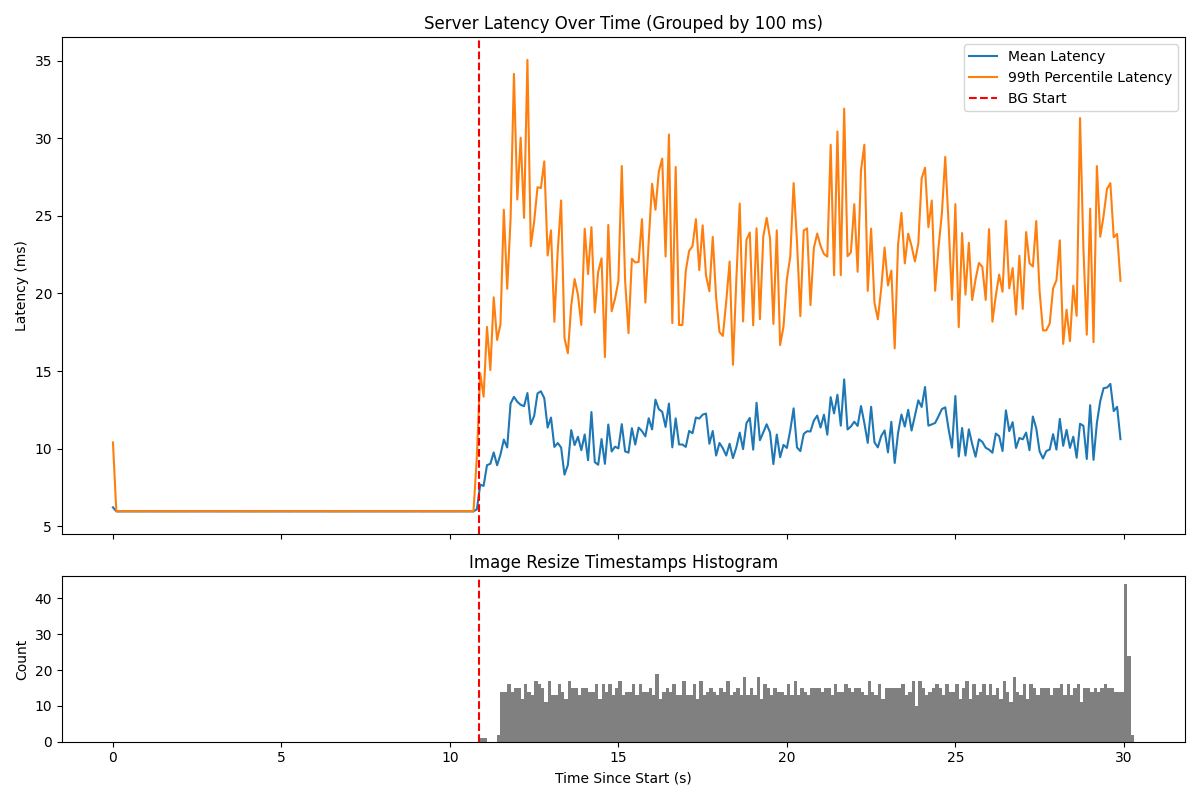
\includegraphics[width=\textwidth]{graphs/unedited-weight-low-two.png}
        \caption{Low load stetting}\label{fig:unedited-weight-low-two}
    \end{subfigure}
    \hspace{\fill}
    \begin{subfigure}[t]{0.48\textwidth}
        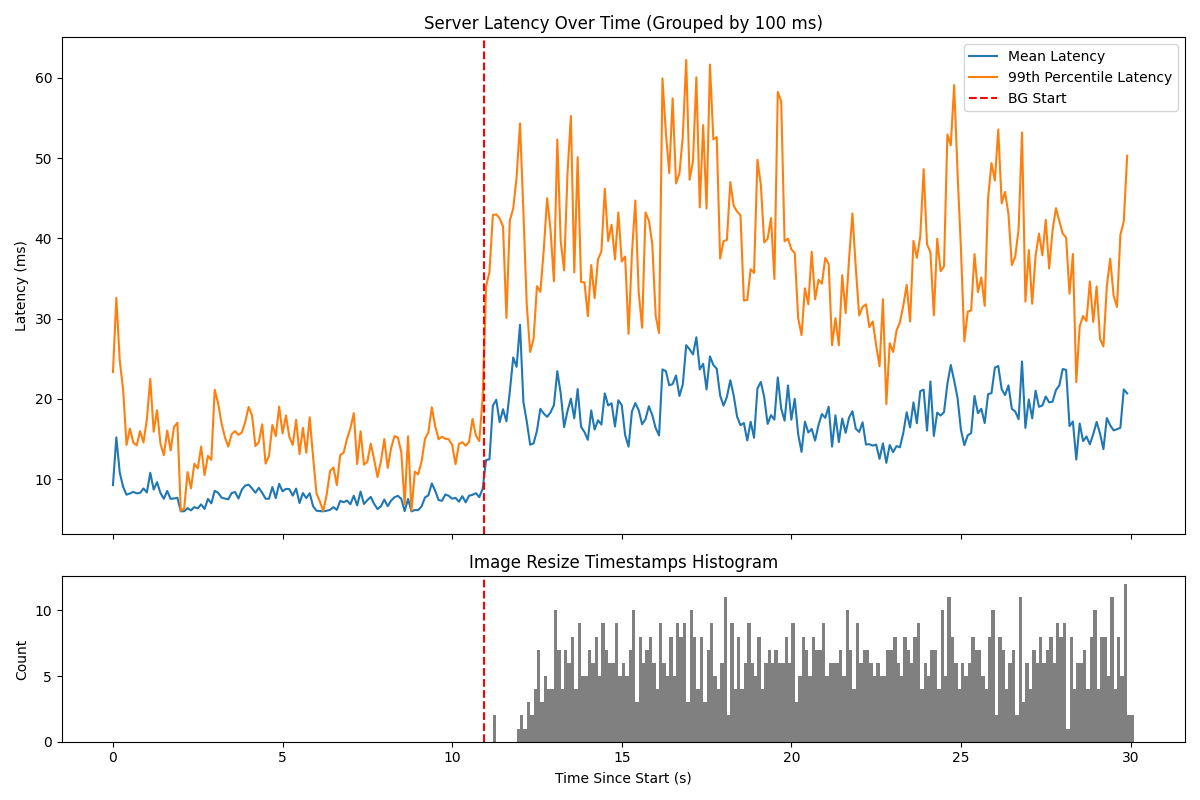
\includegraphics[width=\textwidth]{graphs/unedited-weight-high-two.png}
        \caption{High load setting}\label{fig:unedited-weight-high-two}
    \end{subfigure}
    \caption{Latencies of the server and iteration counts of the background
    tasks in different load scenarios. Note the different y axis limits. The
    upper graphs show end-to-end request latencies, and the bottom graph is a
    histogram of completed iterations of the BE tasks}\label{fig:unedited-weight}
\end{figure*}

In an experiment, we run a (LC) server that processes requests coming in from an
open loop client, running on a separate machine. The client has 100 connections
to the server, each connection creates a new server thread that reads from the
socket and synchronously processes requests in a tight loop. The server threads
run in a cgroup with the highest possible weight: 10000. The server initially
runs on an uncontended four cores, during which time the cpu utilization of the
server is around 85\%. After $\sim$10 seconds, we start two background tasks on
the same four cores, each performing an image resize job. Each background task
is in its own cgroup, which both have the lowest possible weight, 1. We then
measure the latencies experienced by the LC server, before and after starting
the background tasks. Figure~\ref{fig:unedited-weight-low-two} shows the
results. We see that mean latencies spike up from steady at just under 6ms to as
high as 13ms, and much higher for 99th percentile latencies.

With a higher baseline load for the LC server the spikes are higher,
figure~\ref{fig:unedited-weight-high-two} shows the latencies when the
utilization of the uncontended server load is around 95\%.
